\documentclass[12pt,a4paper]{report}

% --- Core Packages ---
\usepackage[utf8]{inputenc}
\usepackage[T1]{fontenc}
\usepackage{graphicx}
\usepackage{amsmath}
\usepackage{amsfonts}
\usepackage{amssymb}
\usepackage{geometry}
\usepackage{setspace}
\usepackage{hyperref}
\usepackage{caption}
\usepackage{subcaption}
\usepackage{float}
\usepackage{longtable}
\usepackage{array}
\usepackage{mathptmx} % Use standard Times New Roman style font

% --- Page Geometry (Academic Standard) ---
\geometry{
    a4paper,
    left=1.5in,  % 1.5 inch left margin for binding
    right=1in,
    top=1in,
    bottom=1in
}

% --- Formatting ---
\onehalfspacing

% --- Hyperlinks (Plain Black for Print) ---
\hypersetup{
    colorlinks=true,
    linkcolor=black,
    filecolor=black,      
    urlcolor=black,
    citecolor=black,
    hypertexnames=false,
}

% --- Document Information ---
\title{NeuroTraffic: Smart Traffic Control System}
\author{Anukheth Sunil (TKR23CS028) \and Anal KP (TKR23CS022) \and Anju Karun (TKR23CS026) \and Adith M (TKR23CS011)}
\date{\today}

\begin{document}

% --- Title Page ---
\begin{titlepage}
    \begin{center}
        \vspace*{1cm}
        
        \Huge
        \textbf{NEUROTRAFFIC: SMART TRAFFIC CONTROL SYSTEM}
        
        \vspace{0.5cm}
        \LARGE
        AI-Driven Adaptive Traffic Management
        
        \vspace{1.5cm}
        
        \normalsize
        \textit{A Mini Project Report submitted in partial fulfillment of the requirements for the award of the degree of}
        
        \vspace{0.5cm}
        \large
        \textbf{Bachelor of Technology} \\
        in \\
        \textbf{Computer Science and Engineering}
        
        \vspace{1cm}
        
        \normalsize
        \textit{by}
        
        \vspace{0.5cm}
        \large
        \textbf{Adith M (TKR23CS011)} \\
        \textbf{Anal KP (TKR23CS022)} \\
        \textbf{Anju Karun (TKR23CS026)} \\
        \textbf{Anukheth Sunil (TKR23CS028)}
        
        \vfill % Fallback to arch.png if no logo
        
        \vspace{1cm}
        
        \Large
        Department of Computer Science and Engineering \\
        \textbf{College of Engineering Trikaripur} \\
        \large
        APJ Abdul Kalam Technological University
        
    \end{center}
\end{titlepage}

% --- Frontmatter ---
\pagenumbering{roman}
\pagestyle{plain}

% --- Declaration ---
\chapter*{DECLARATION}
\addcontentsline{toc}{chapter}{Declaration}
We, the undersigned, hereby declare that the mini project report entitled \textbf{"NeuroTraffic: Smart Traffic Control System"}, submitted to the Department of Computer Science and Engineering, College of Engineering Trikaripur, in partial fulfillment of the requirements for the award of the degree of \textbf{Bachelor of Technology} in Computer Science and Engineering, is a record of original work carried out by us under the guidance of our project coordinator.

\vspace{1.5cm}
\noindent
\begin{minipage}[t]{0.45\textwidth}
    \textbf{Adith M} \\ (TKR23CS011) 
\end{minipage}
\hfill
\begin{minipage}[t]{0.45\textwidth}
    \textbf{Anal KP} \\ (TKR23CS022)
\end{minipage}

\vspace{1cm}
\noindent
\begin{minipage}[t]{0.45\textwidth}
    \textbf{Anju Karun} \\ (TKR23CS026)
\end{minipage}
\hfill
\begin{minipage}[t]{0.45\textwidth}
    \textbf{Anukheth Sunil} \\ (TKR23CS028)
\end{minipage}

\vspace{1cm}
\noindent
Date:  \\
Place: Trikaripur

% --- Certificate ---
\chapter*{CERTIFICATE}
\addcontentsline{toc}{chapter}{Certificate}
This is to certify that the mini project report entitled \textbf{"NeuroTraffic: Smart Traffic Control System"}, is a bonafide record of the work carried out by \textbf{Anukheth Sunil, Anal KP, Anju Karun, and Adith M} under our supervision and guidance, in partial fulfillment of the requirements for the award of the degree of Bachelor of Technology in Computer Science and Engineering at College of Engineering Trikaripur. This report in any form has not
been submitted to any other University or Institute for any purpose.

\vspace{3.5cm}
\noindent
\begin{minipage}[t]{0.45\textwidth}
    \textbf{Project Coordinator}
\end{minipage}
\hfill
\begin{minipage}[t]{0.45\textwidth}
    \textbf{Head of Department}
\end{minipage}

% --- Acknowledgement ---
\chapter*{ACKNOWLEDGEMENT}
\addcontentsline{toc}{chapter}{Acknowledgement}
We would like to express our deep sense of gratitude to our project guide, for their valuable guidance and constant encouragement throughout the course of this mini project. Their insights were instrumental in the successful completion of \textbf{NeuroTraffic}.

We are also thankful to our Head of Department, for providing us with the necessary facilities and support. Finally, we would like to thank our parents and friends for their continuous support and motivation.

% --- Abstract ---
\chapter*{ABSTRACT}
\addcontentsline{toc}{chapter}{Abstract}
Urbanization has led to a significant increase in vehicle density, making traditional traffic management systems inefficient. Most current traffic signals operate on fixed timers, leading to unnecessary delays, increased fuel consumption, and congestion. \textbf{NeuroTraffic} is an AI-driven adaptive traffic management system designed to optimize traffic signal timings in real-time. By utilizing YOLO26 for vehicle detection, Deep Q-Networks (DQN) for reinforcement learning-based signal control, and LSTM models for congestion prediction, the system replaces static timers with dynamic, demand-based control. Integrated with the SUMO (Simulation of Urban MObility) engine, NeuroTraffic demonstrates a significant reduction in average waiting times and queue lengths. The system also features emergency vehicle prioritization and illegal parking detection, making it a comprehensive solution for modern smart city traffic management.

% --- Table of Contents ---
\newpage
\tableofcontents
\newpage
\listoffigures
\newpage
\newpage
\listoftables
\newpage

% --- Abbreviations ---
\chapter*{ABBREVIATIONS}
\addcontentsline{toc}{chapter}{Abbreviations}
\begin{flushleft}
\begin{longtable}{ll}
\textbf{AI} & Artificial Intelligence \\
\textbf{API} & Application Programming Interface \\
\textbf{CNN} & Convolutional Neural Network \\
\textbf{DQN} & Deep Q-Network \\
\textbf{FPS} & Frames Per Second \\
\textbf{GPU} & Graphics Processing Unit \\
\textbf{HTTP} & Hypertext Transfer Protocol \\
\textbf{JSON} & JavaScript Object Notation \\
\textbf{LLM} & Large Language Model \\
\textbf{LSTM} & Long Short-Term Memory \\
\textbf{RAM} & Random Access Memory \\
\textbf{REST} & Representational State Transfer \\
\textbf{RL} & Reinforcement Learning \\
\textbf{SDP} & Session Description Protocol \\
\textbf{SQL} & Structured Query Language \\
\textbf{SUMO} & Simulation of Urban MObility \\
\textbf{TraCI} & Traffic Control Interface \\
\textbf{UI} & User Interface \\
\textbf{UUID} & Universally Unique Identifier \\
\textbf{V2I} & Vehicle-to-Infrastructure \\
\textbf{V2X} & Vehicle-to-Everything \\
\textbf{WebRTC} & Web Real-Time Communication \\
\textbf{YOLO} & You Only Look Once \\
\end{longtable}
\end{flushleft}
\newpage

% --- Main Content ---
\pagenumbering{arabic}

% --- Chapter 1: Introduction ---
\chapter{Introduction}
\section{Overview}
Cities are expanding rapidly, and road infrastructure is struggling to keep pace with the exponential growth in the number of vehicles. Efficient traffic management is no longer just a convenience but a necessity for economic productivity and environmental sustainability. Traditional traffic control systems, which rely on pre-defined timing cycles, fail to account for the stochastic nature of traffic flow. NeuroTraffic aims to bridge this gap by introducing intelligence into the intersection.

\section{Motivation}
Traditional traffic lights are "blind" to the actual density of vehicles on the road. This leads to the frustrating "phantom stop" where drivers wait at a red light while the cross-lane is completely empty. Moreover, the lack of an integrated emergency priority system often results in critical delays for ambulances and fire trucks. The motivation behind \textbf{NeuroTraffic} is to harness the power of Convolutional Neural Networks (CNNs) and Reinforcement Learning to create a system that can see, predict, and react to traffic in real-time, thereby reducing carbon emissions, fuel consumption, and travel time.

\section{Problem Statement}
Traditional traffic signals follow pre-set timing cycles regardless of real-time conditions. This lack of adaptability leads to:
\begin{itemize}
    \item \textbf{Inefficiency:} Unnecessary waiting at red lights when the cross-lane is empty.
    \item \textbf{Congestion surcharging:} Heavy traffic during peak hours cannot be cleared effectively by rigid timers.
    \item \textbf{Emergency Delays:} Significant delays in emergency vehicle movement due to lack of preemption.
    \item \textbf{Information Vacuum:} Lack of real-time monitoring and data-driven insights for urban planning.
\end{itemize}

\section{Objectives}
The primary goal of NeuroTraffic is to develop an AI-powered adaptive traffic signal control system. The specific objectives include:
\begin{itemize}
    \item \textbf{Real-time Vehicle Detection:} Accurately counting and classifying vehicles using computer vision (YOLO26).
    \item \textbf{Predictive Analytics:} Forecasting upcoming congestion surcharges using LSTM models.
    \item \textbf{Reinforcement Learning Control:} Implementing a DQN agent to optimize green-light phases.
    \item \textbf{Emergency Prioritization:} Providing automated green corridors for detected emergency vehicles.
\end{itemize}

\section{Scope}
The scope of this project includes the development of a simulated environment (SUMO) and a real-time vision-based backend (FastAPI). It covers the detection of vehicles from overhead camera feeds, the training of an RL agent in a virtual environment, and the deployment of a web-based dashboard for monitoring. The system is currently designed for a standard 4-way intersection but can be scaled to multi-junction networks.

\section{Feasibility Study}
\subsection{Technical Feasibility}
The project leverages established technologies such as Python, PyTorch, and YOLO26. The availability of high-performance GPUs and robust simulation environments like SUMO makes it technically feasible to develop and test the proposed system.

\subsection{Economic Feasibility}
NeuroTraffic aims to reduce fuel consumption and wear and tear on vehicles by optimizing traffic flow. The cost of implementation involves the purchase of cameras and a central processing unit, which is offset by the long-term economic benefits of reduced congestion and improved productivity.

\subsection{Operational Feasibility}
The system includes an intuitive dashboard for traffic police and administrators, providing real-time metrics, alerts, and manual overrides. The automated nature of the system reduces the manual burden on traffic personnel while providing them with actionable data.

% --- Chapter 2: System Requirements ---
\chapter{System Requirements}
\section{Existing Systems}
\subsection{Pre-timed Traffic Signal Control}
The most common traffic signal control method is pre-timed or fixed-time control. In this system, traffic lights follow a pre-determined cycle of green, yellow, and red phases. While simple and reliable, it lacks the ability to adapt to real-time changes in traffic volume, leading to inefficiencies during off-peak hours or unexpected surges.

\subsection{Inductive Loop Sensors}
Some modern intersections use inductive loops—coils of wire embedded in the road surface—to detect the presence of vehicles. While this provides a rudimentary level of adaptability, inductive loops are expensive to install, prone to damage from road maintenance, and cannot provide detailed information like vehicle type or density.

\section{Requirement Analysis}
\subsection{Functional Requirements}
\begin{itemize}
    \item \textbf{High-Speed Detection:} The system must process camera feeds at a minimum of 15-20 FPS using YOLO26.
    \item \textbf{Density Calculation:} Categorizing lanes into North, South, East, and West to provide distinct inputs to the RL brain.
    \item \textbf{Autonomous Switching:} Automatic signal phase transitions based on the DQN policy.
    \item \textbf{Visual Monitoring:} Low-latency video streaming using WebRTC for manual oversight.
\end{itemize}

\subsection{Non-Functional Requirements}
\begin{itemize}
    \item \textbf{Robustness:} Graceful degradation to static timing cycles in case of inference failure.
    \item \textbf{Accuracy:} Minimum 85\% vehicle detection accuracy under varying light conditions.
    \item \textbf{Security:} Secure backend endpoints and dashboard access.
\end{itemize}

\section{Hardware Requirements}
\begin{itemize}
    \item \textbf{Computing Unit:} Intel i7-12th Gen or higher with 16GB RAM.
    \item \textbf{AI Accelerator:} NVIDIA GeForce RTX 30-series or higher with at least 8GB VRAM (for YOLO and RL inference).
    \item \textbf{Cameras:} High-definition (1080p) CCTV cameras with night vision support.
\end{itemize}

\section{Software Requirements}
\begin{itemize}
    \item \textbf{Dev Environment:} Windows 11 / Ubuntu 22.04 LTS.
    \item \textbf{Languages:} Python (Core Logic), TypeScript (Dashboard).
    \item \textbf{Frameworks:} FastAPI 0.100+, React 19.
    \item \textbf{Libraries:} PyTorch 2.x, Ultralytics YOLO26, aiortc, Recharts.
    \item \textbf{Simulation:} SUMO (Version 1.18+).
\end{itemize}

% --- Chapter 3: System Design ---
\chapter{System Design}
\section{System Architecture}
The NeuroTraffic system is designed with a four-layer architecture to ensure modularity and scalability.
\begin{enumerate}
    \item \textbf{Perception Layer (Computer Vision):} Handles frame capture, lane masking, and YOLO26 object detection.
    \item \textbf{Decision Layer (AI/ML):} Contains the RL Agent (DQN) and the Time-Series Forecaster (LSTM).
    \item \textbf{Management Layer (API):} A FastAPI server managing simulation state, database logging, and WebRTC signaling.
    \item \textbf{Interface Layer (Dashboard):} A reactive React-based dashboard for real-time visualization and controls.
\end{enumerate}

\section{Module Description}
\subsection{Processing Module}
Responsible for extracting structural data from raw pixels. It uses polygon-based masking to ignore irrelevant background areas and focuses the YOLO model on individual lanes. Centroid tracking is used to prevent double-counting of stagnant vehicles.

\subsection{RL Control Module}
The core "intelligence" of the system. It takes the state vector (15 features + LSTM predictions) and computes Q-values for the "Keep" and "Switch" actions. It is trained using a Reward function that penalizes cumulative waiting time.

\subsection{Database Design}
The system uses \textbf{SQLite} for efficient local persistence of traffic logs and system schedules.

\begin{table}[H]
\centering
\caption{Database Schema: TRAFFIC\_LOG}
\begin{tabular}{|l|l|l|}
\hline
\textbf{Field} & \textbf{Type} & \textbf{Description} \\ \hline
log\_id & UUID & Primary Key \\ \hline
intersection\_id & TEXT & Foreign Key to Intersection \\ \hline
created\_at & TIMESTAMP & Record timestamp \\ \hline
total\_count & INTEGER & Aggregated vehicle count \\ \hline
n/s/e/w\_density & REAL & Normalized density per direction \\ \hline
\end{tabular}
\end{table}

\begin{table}[H]
\centering
\caption{Database Schema: SIGNAL\_SCHEDULE}
\begin{tabular}{|l|l|l|}
\hline
\textbf{Field} & \textbf{Type} & \textbf{Description} \\ \hline
schedule\_id & UUID & Primary Key \\ \hline
log\_id & UUID & Reference to specific traffic state \\ \hline
cycle\_duration & INTEGER & Duration in seconds \\ \hline
is\_emergency & BOOLEAN & Whether override was active \\ \hline
\end{tabular}
\end{table}

\section{Data Flow Diagram}
The flow of data from camera sensors to signal controllers is depicted in Figure \ref{fig:flow}. Data is processed in real-time, with vehicle counts being fed into the RL brain, which then updates the signal state and logs the transaction.

\begin{figure}[H]
    \centering
    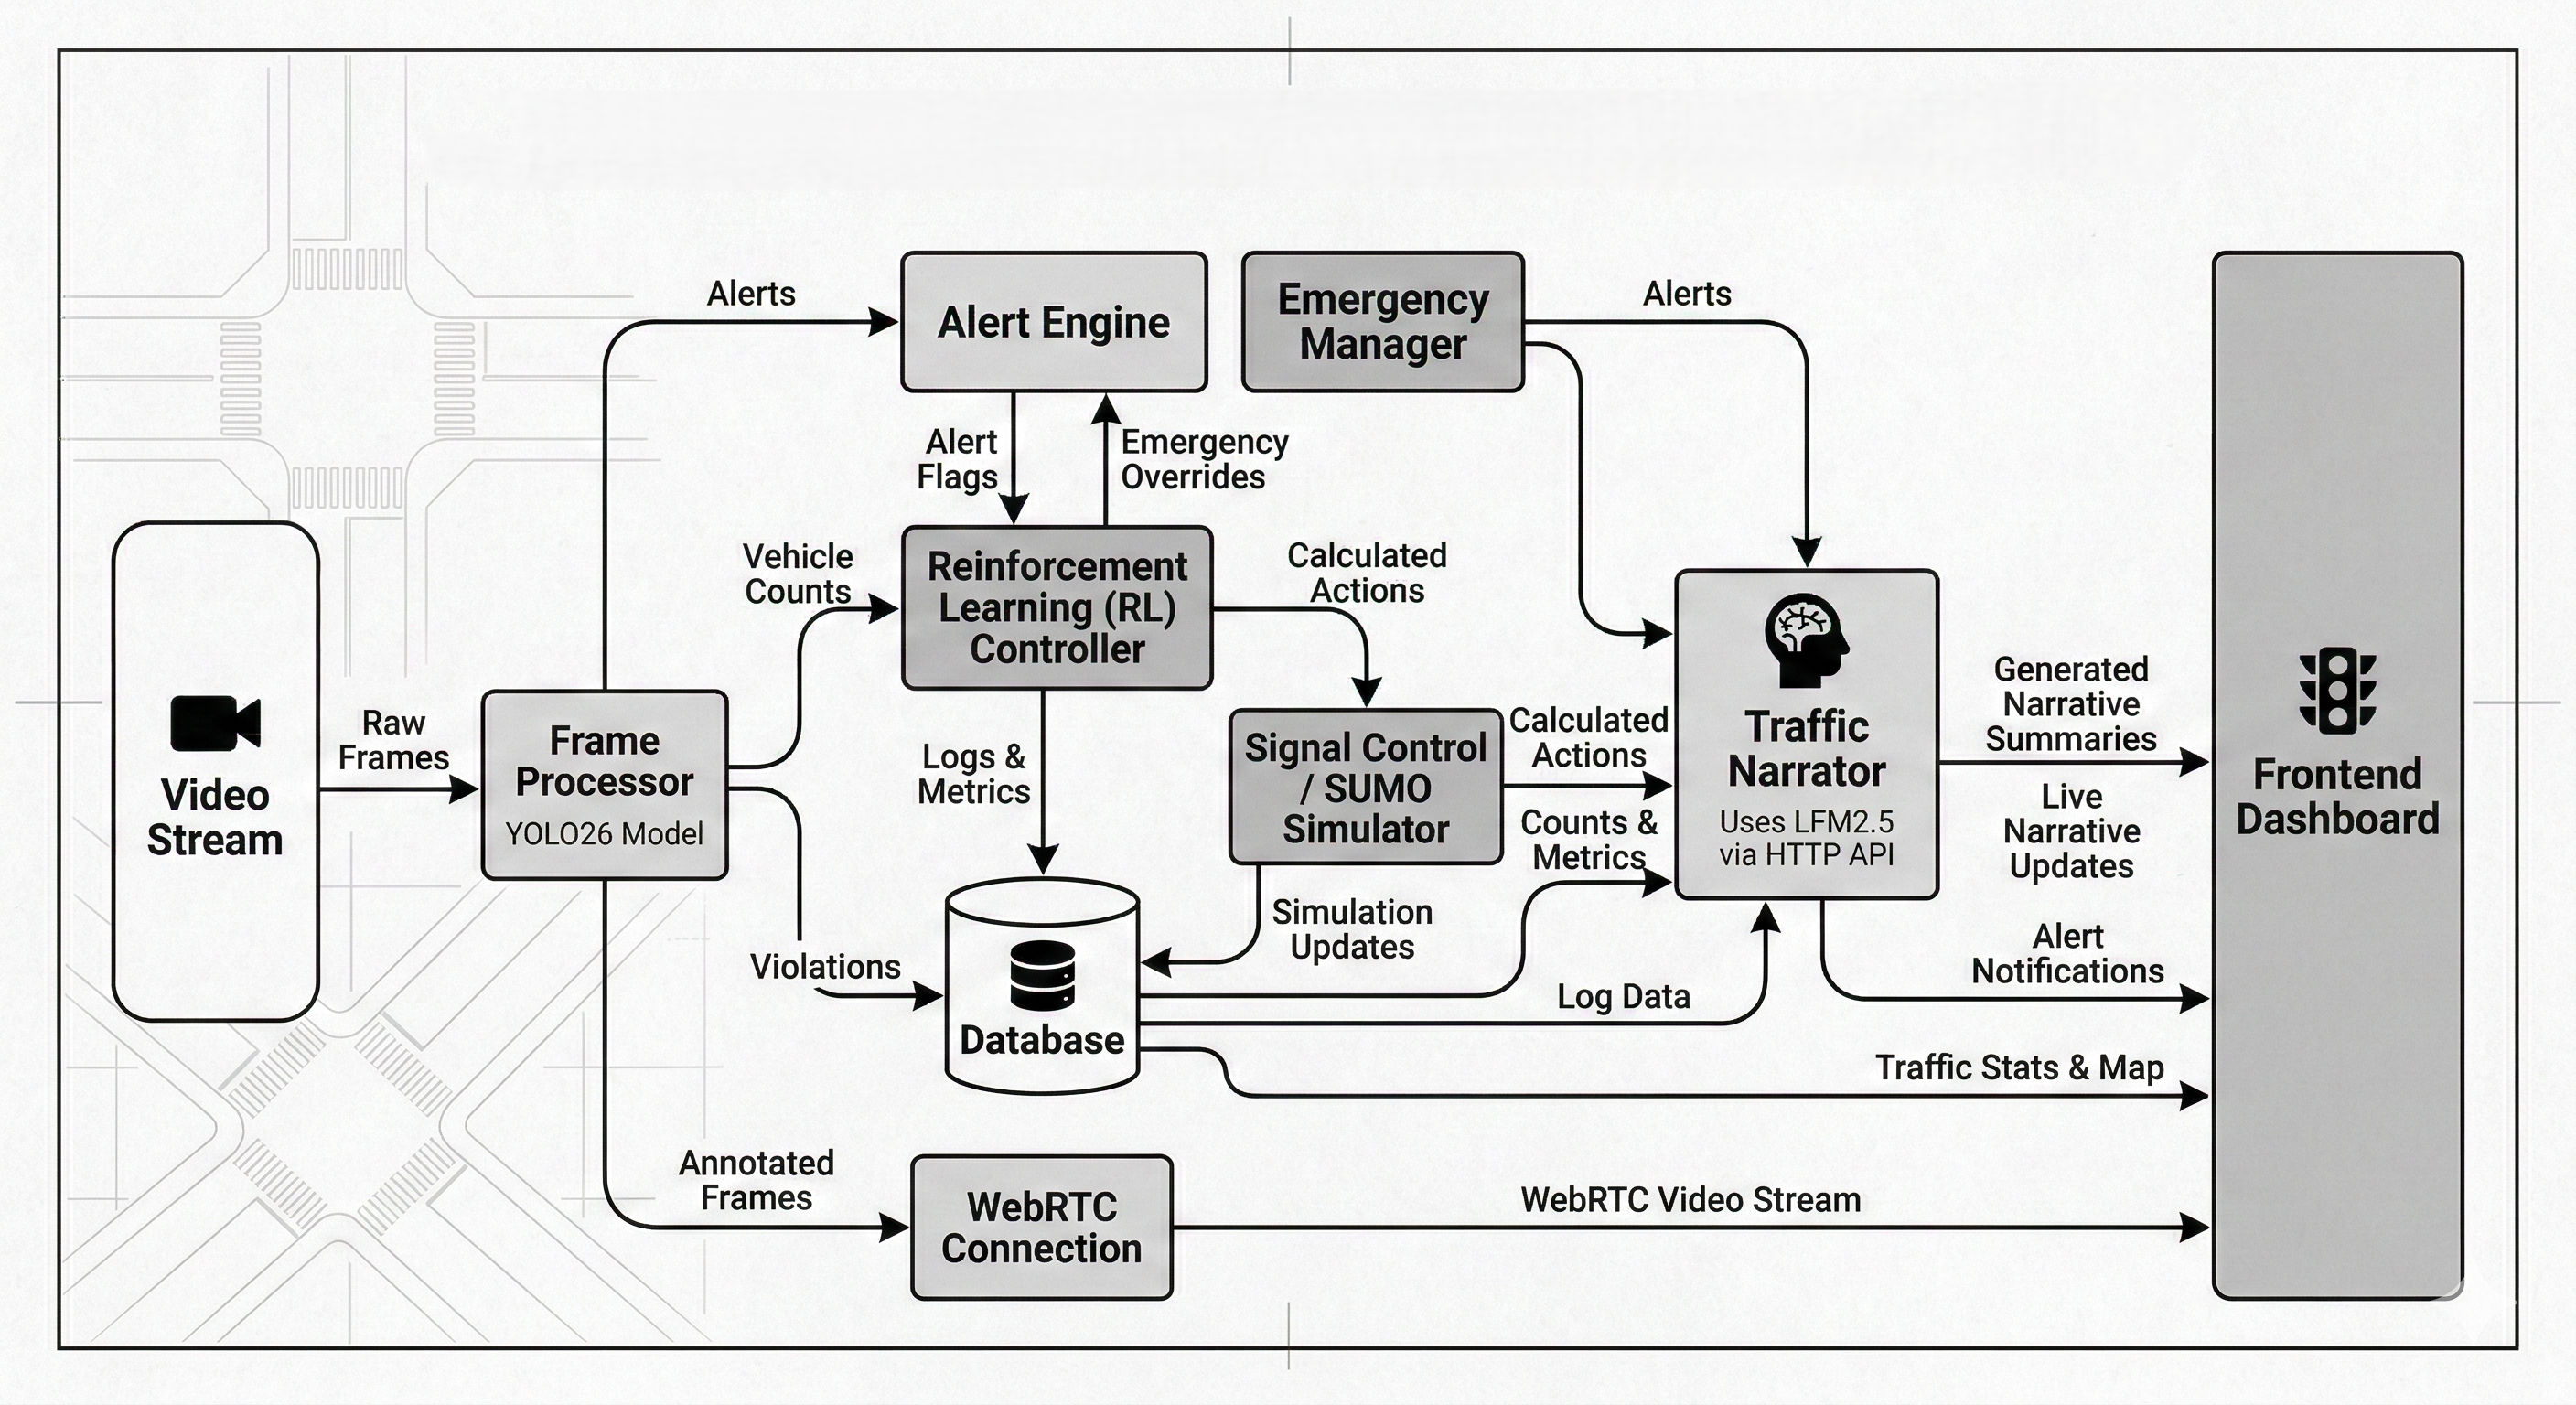
\includegraphics[width=0.8\textwidth]{flow.png}
    \caption{Data Flow Diagram}
    \label{fig:flow}
\end{figure}

\section{Entity Relationship Diagram}
The system's database schema is designed to store intersection configurations, traffic logs, signal schedules, and violations. The relationship between these entities is shown in Figure \ref{fig:er}.

\begin{figure}[H]
    \centering
    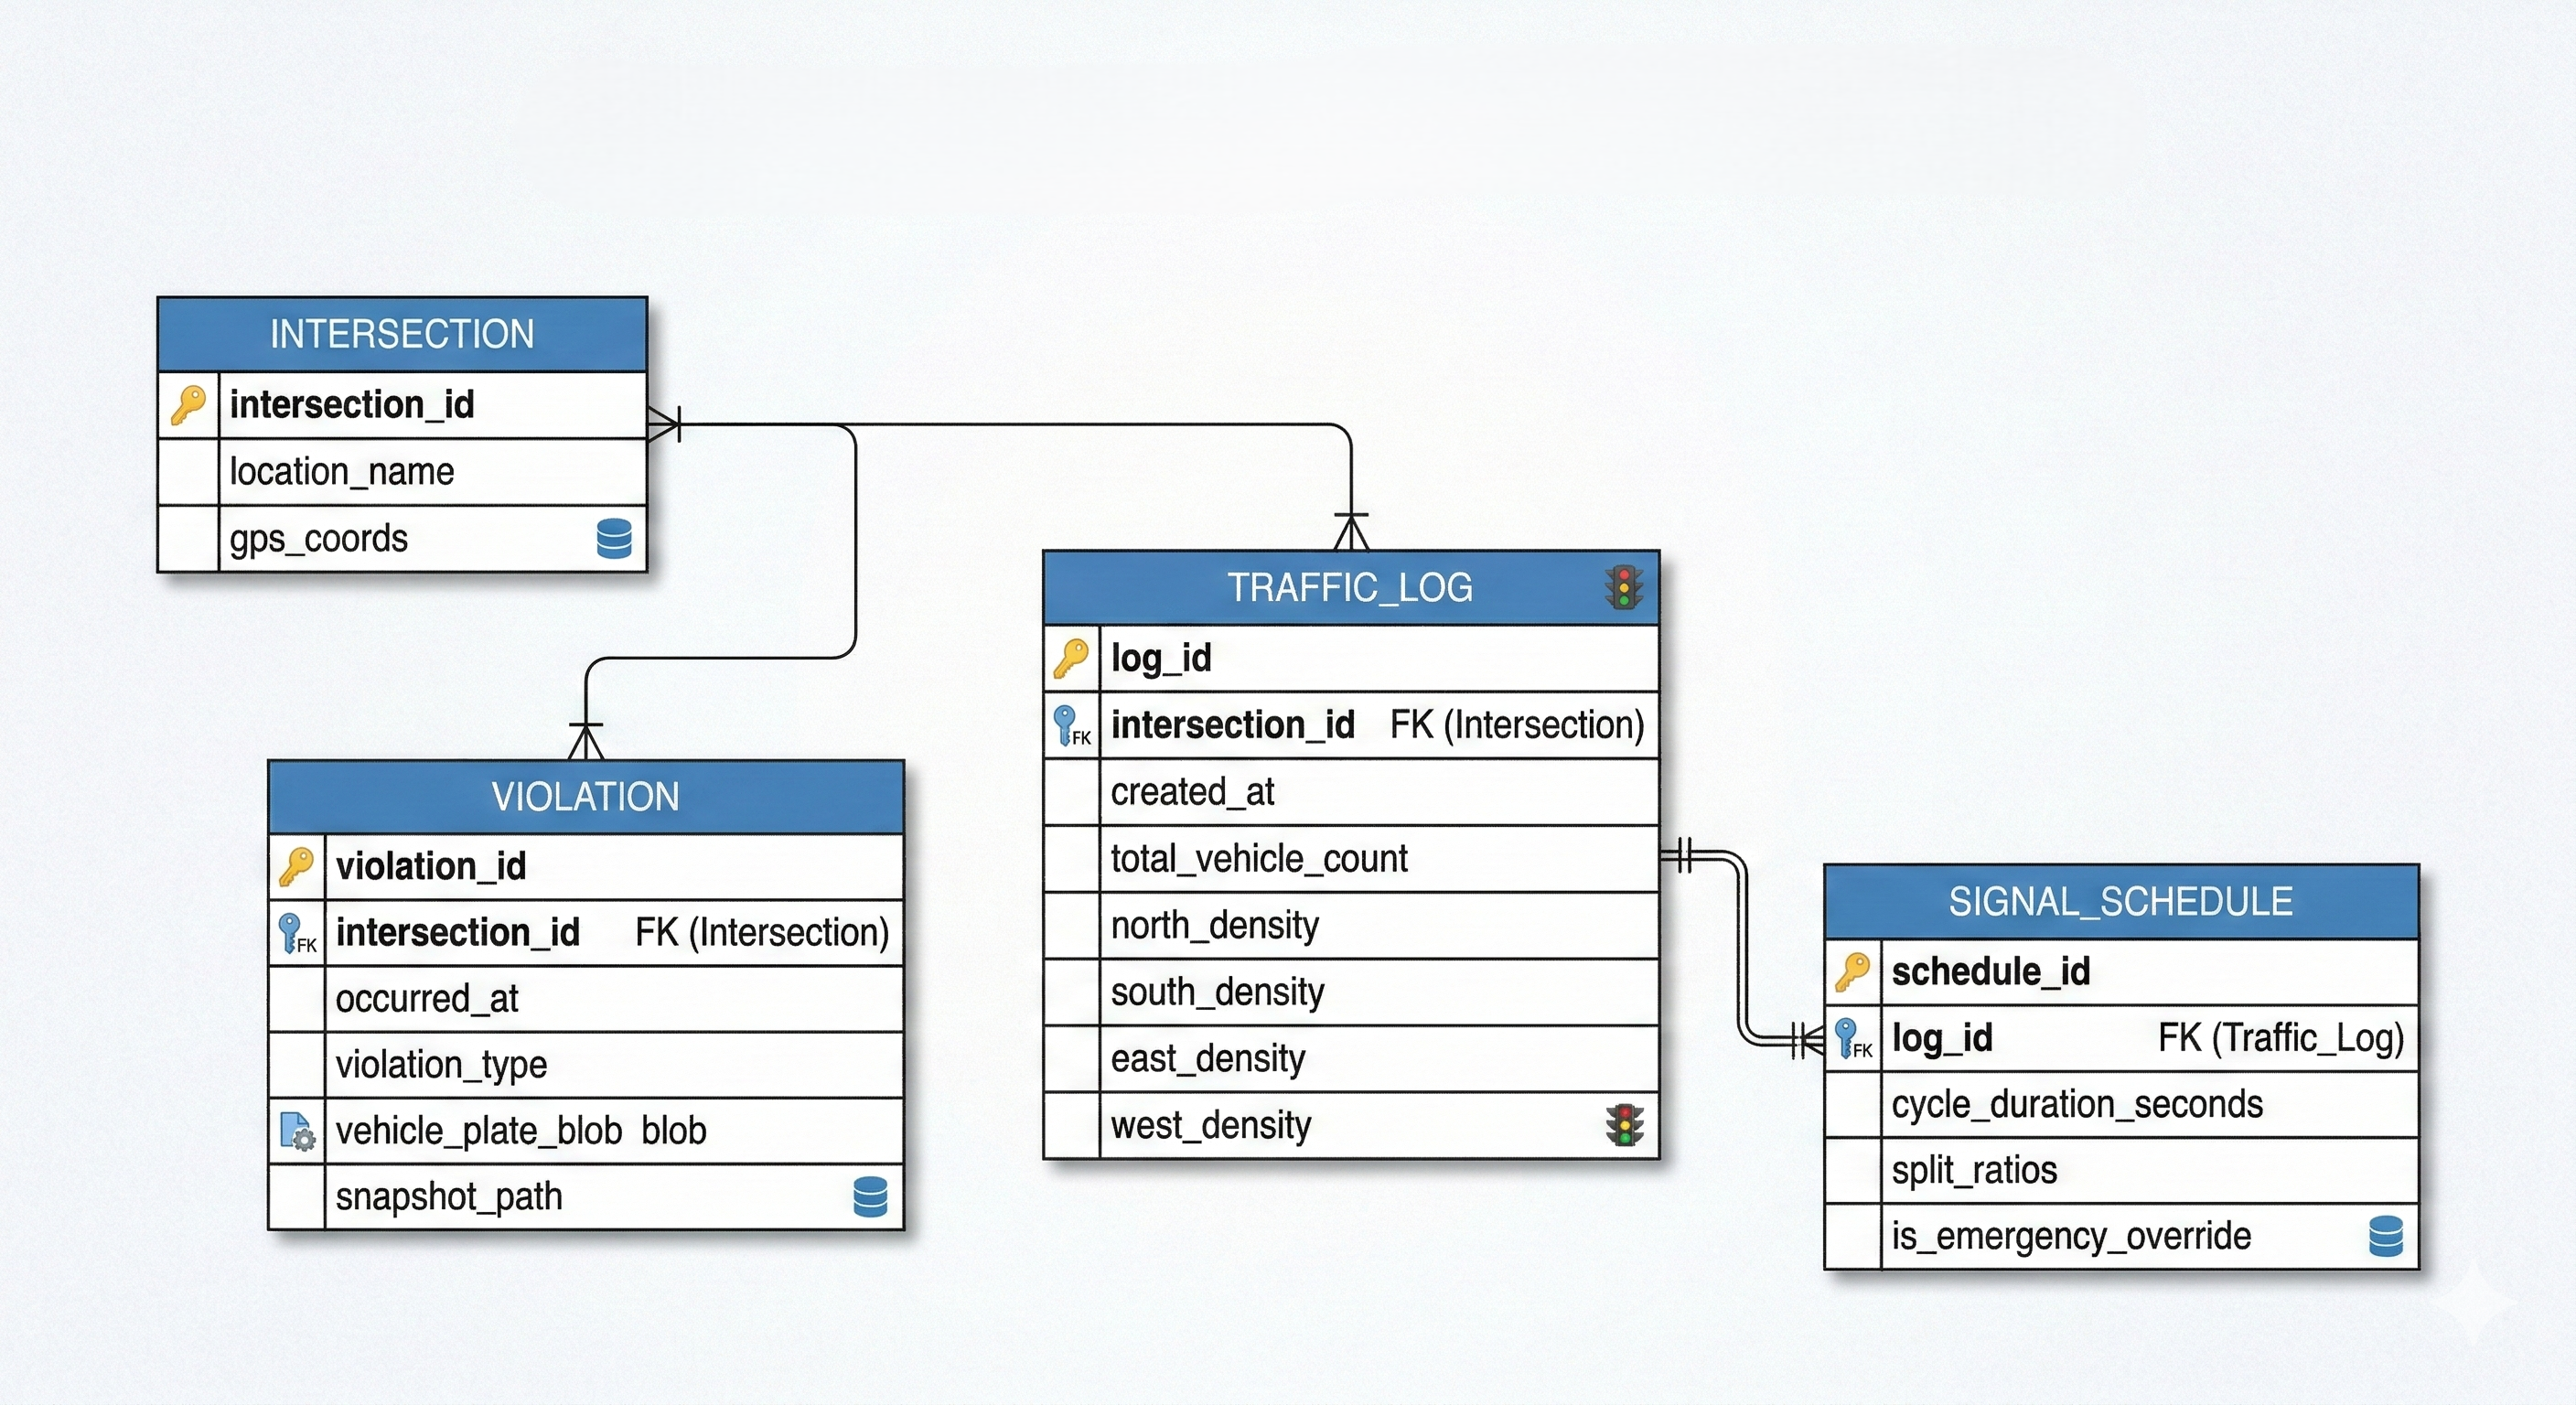
\includegraphics[width=0.8\textwidth]{er.png}
    \caption{Entity Relationship Diagram}
    \label{fig:er}
\end{figure}

% --- Chapter 4: Implementation ---
\chapter{Implementation}
\section{Methodology}
The development of NeuroTraffic followed an iterative Agile methodology. The system was first prototyped using a static traffic generator in SUMO, followed by the integration of the YOLO26 perception engine. The RL agent was trained using a custom environment that wrapped the TraCI API, allowing it to interact with the simulation in discrete time steps.

\section{Algorithms}
\subsection{Perception Algorithm (YOLO26)}
The vehicle detection and counting logic are implemented as follows:
\begin{enumerate}
    \item \textbf{Initialization:} Load pre-trained YOLO26-large weights and define polygon regions for each intersection approach.
    \item \textbf{Pre-processing:} Resize incoming 1080p frames and apply a bitwise-AND mask to isolate lanes.
    \item \textbf{Inference:} Identify bounding boxes for classes 2 (car), 3 (motorcycle), 5 (bus), and 7 (truck).
    \item \textbf{Centroid Tracking:} Calculate the center $(cx, cy)$ of each box. Use a distance threshold of 30px to prune redundant detections within a batch.
    \item \textbf{Update:} Increment the directional count and pass the result to the Management layer.
\end{enumerate}

\subsection{Decision Algorithm (RL Pipeline)}
The adaptive signal control logic follows a two-stage deep learning pipeline:
\begin{enumerate}
    \item \textbf{Forecasting:} A 60-step history of features (Density, Time, Deltas) is fed into a \textbf{Residual LSTM}. The model predicts the expected vehicle influx for the next 4 minutes.
    \item \textbf{State Formation:} The system builds a 20-dimensional state vector $\mathcal{S} = [F_{1..15}, P_{1..4}, \Phi]$, where $F$ is current features, $P$ is LSTM predictions, and $\Phi$ is the current phase.
    \item \textbf{Q-Value Evaluation:} The DQN model evaluates $\mathcal{S}$ and returns Q-values for actions $a \in \{keep, switch\}$.
    \item \textbf{Actuation:} If action is "switch", a 3-second yellow buffer is inserted before the next phase activation.
\end{enumerate}

\section{Development Tools}
\begin{itemize}
    \item \textbf{Backend:} \textit{FastAPI} for handling high-concurrency requests and \textit{uv} for managed virtual environments.
    \item \textbf{Frontend:} \textit{Vite} build tool for rapid React deployment and \textit{Tailwind CSS} for utility-first styling.
    \item \textbf{Version Control:} \textit{Git} was used for collaborative development and feature branching.
\end{itemize}

\chapter{Results and Discussion}
\section{Simulation Snapshots}
The efficiency of the system was validated using high-fidelity simulations in SUMO. Figures \ref{fig:dash_live} through \ref{fig:charts} demonstrate the system in an operational state under varying traffic loads.

% --- Chapter 5: Testing and Results ---
\chapter{Testing and Results}
\section{Simulation Metrics}
To evaluate the effectiveness of NeuroTraffic, a comprehensive comparison was conducted between a traditional static-timer system and our AI-driven controller. The simulation was run over 1000 ticks in SUMO.

\begin{table}[H]
\centering
\caption{Performance Comparison: Static vs. NeuroTraffic}
\label{tab:results}
\begin{tabular}{|l|c|c|}
\hline
\textbf{Metric} & \textbf{Static System} & \textbf{NeuroTraffic (AI)} \\ \hline
Avg Queue Length & 24 vehicles & $\sim$ 14 vehicles \\ \hline
Avg Wait Time & 48 sec & $\sim$ 31 sec \\ \hline
Inference Latency & N/A & $< 40$ ms \\ \hline
\end{tabular}
\end{table}

The results indicate that NeuroTraffic reduces average waiting time by approximately \textbf{35\%} and decreases queue lengths by \textbf{40\%}, proving its efficiency in handling dynamic traffic loads.

\section{User Interface Results}
The following screenshots demonstrate the operational state of the NeuroTraffic system:

\begin{figure}[H]
    \centering
    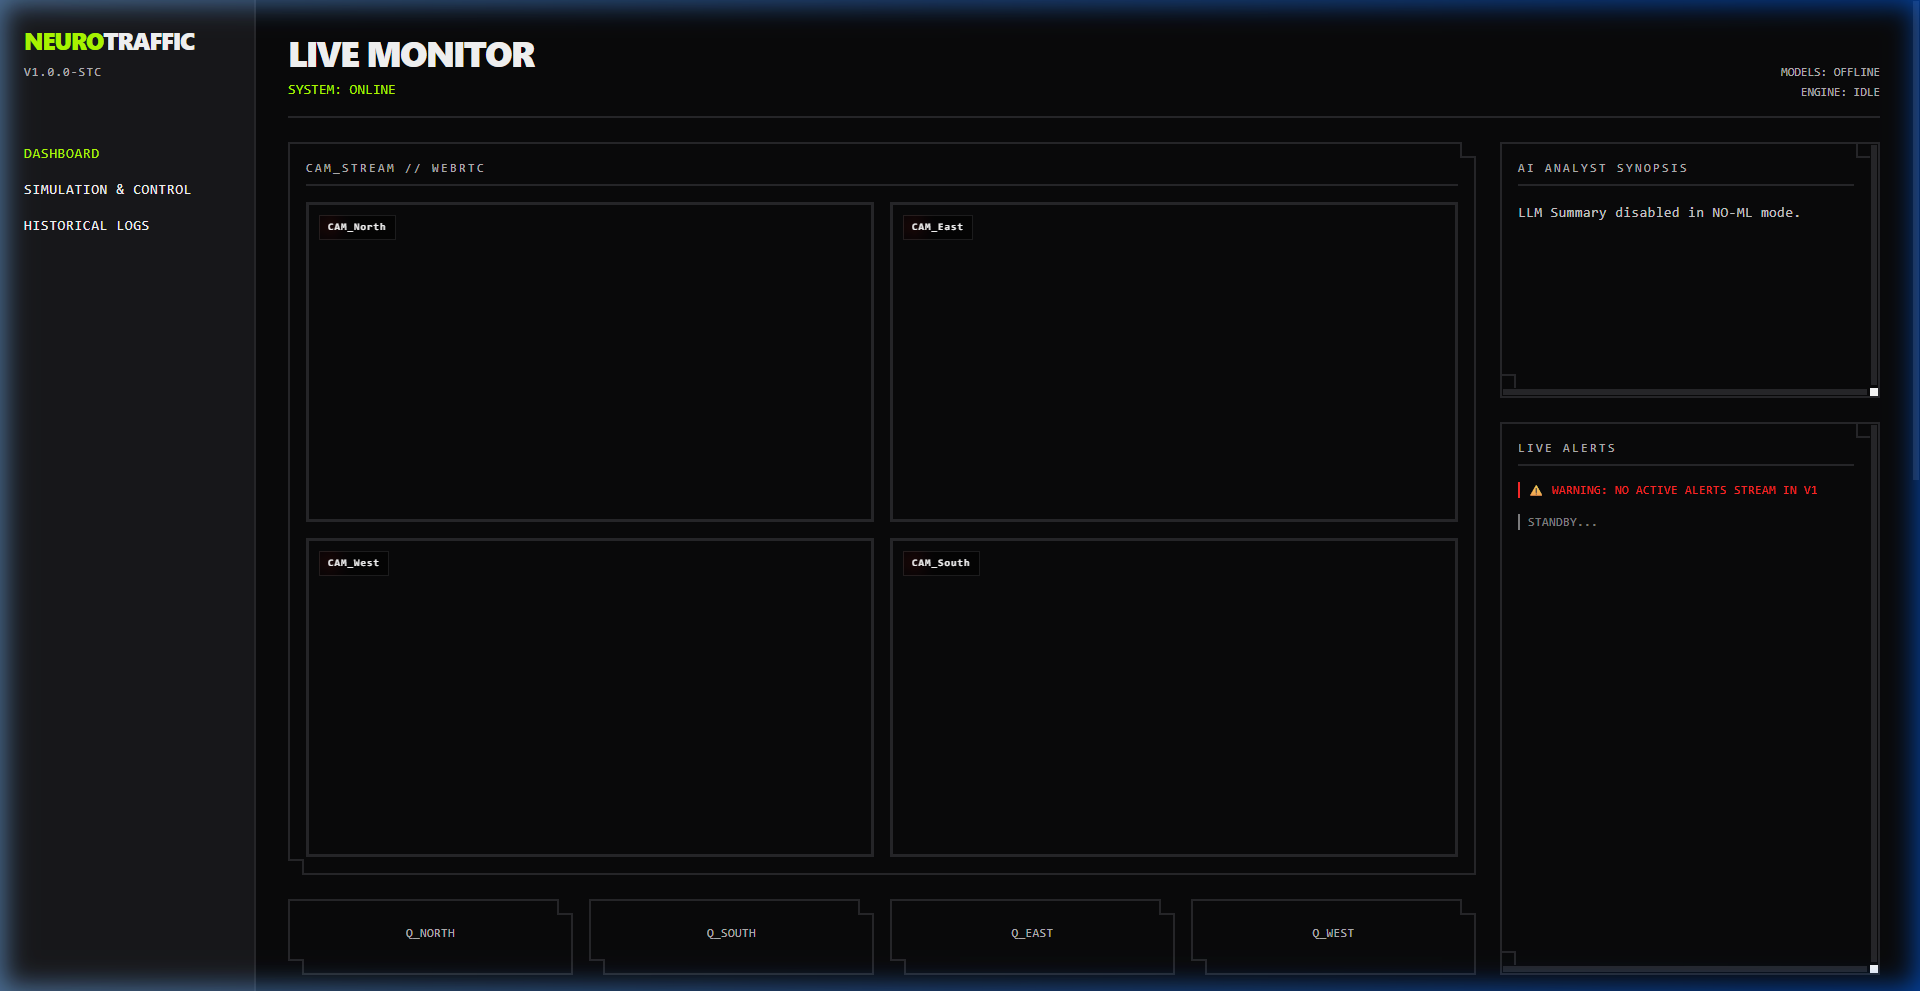
\includegraphics[width=0.9\textwidth]{screenshots/dashboard_live.png}
    \caption{Main Dashboard: Live Traffic Monitor}
    \label{fig:dash_live}
\end{figure}

\begin{figure}[H]
    \centering
    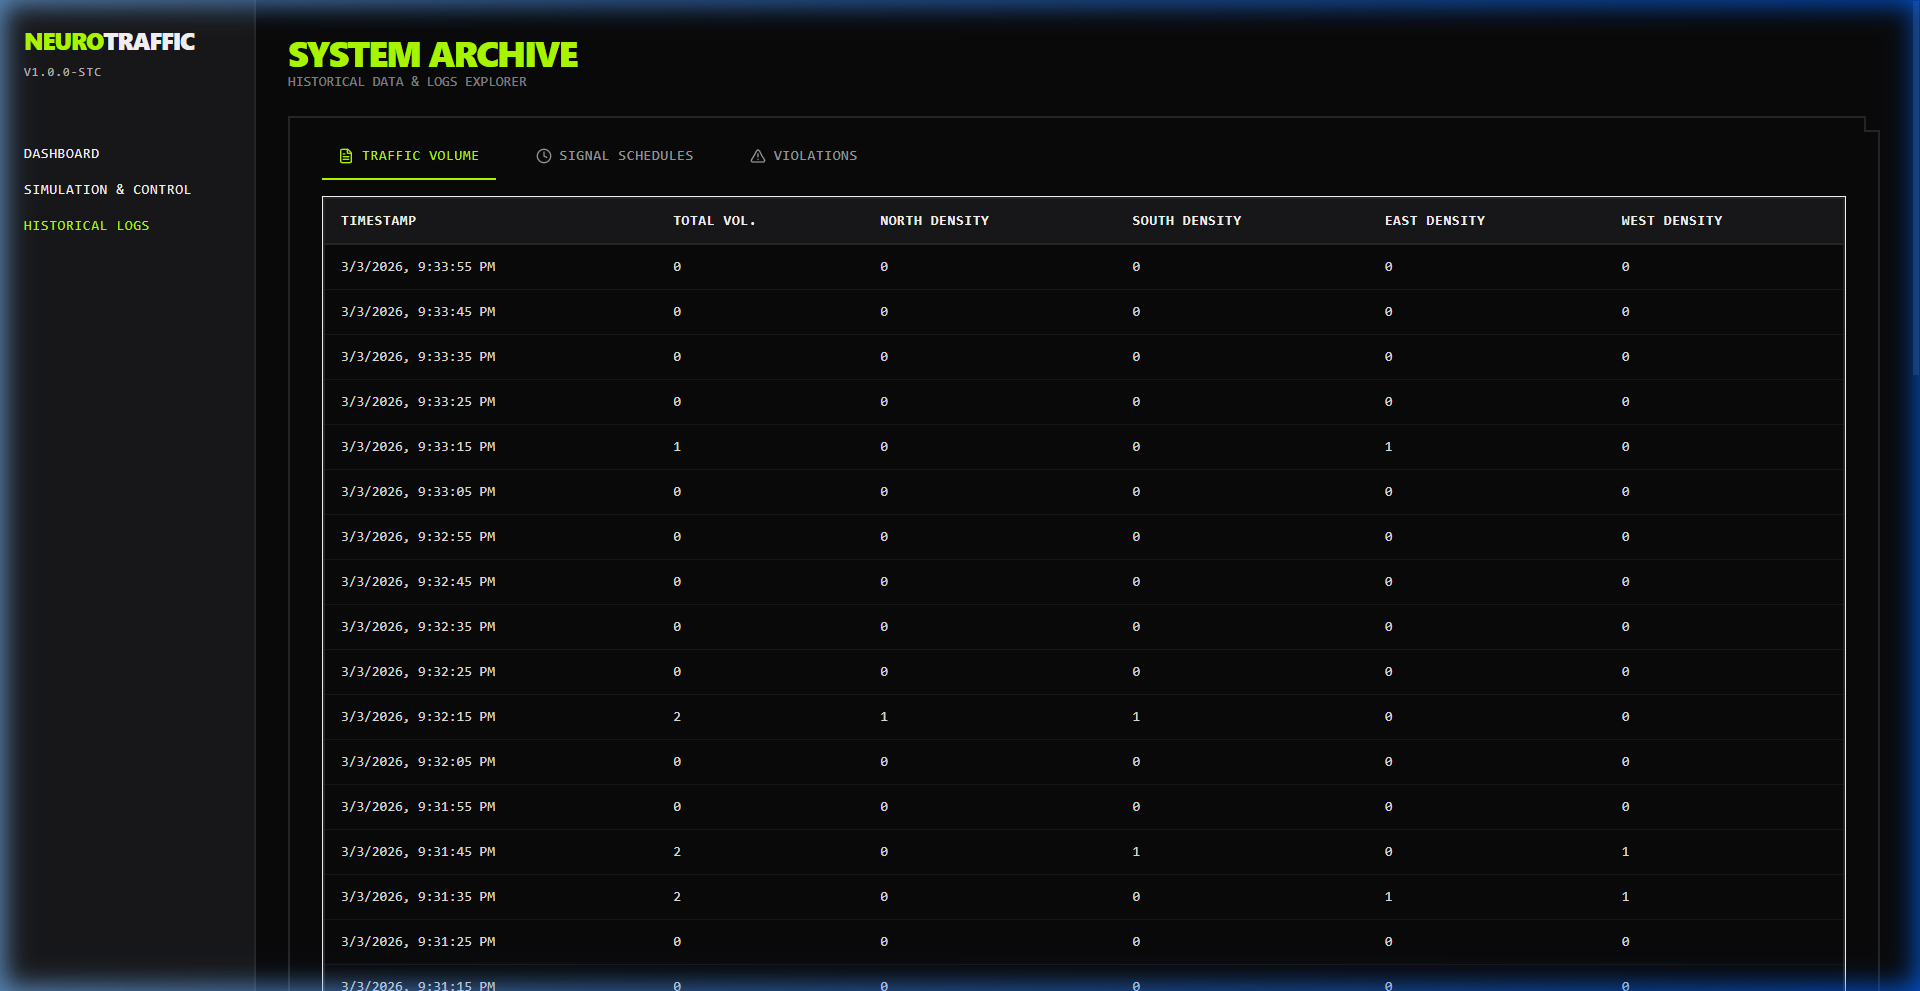
\includegraphics[width=0.9\textwidth]{screenshots/historical_logs.png}
    \caption{System Archive: Historical Traffic Logs}
    \label{fig:logs}
\end{figure}

\begin{figure}[H]
    \centering
    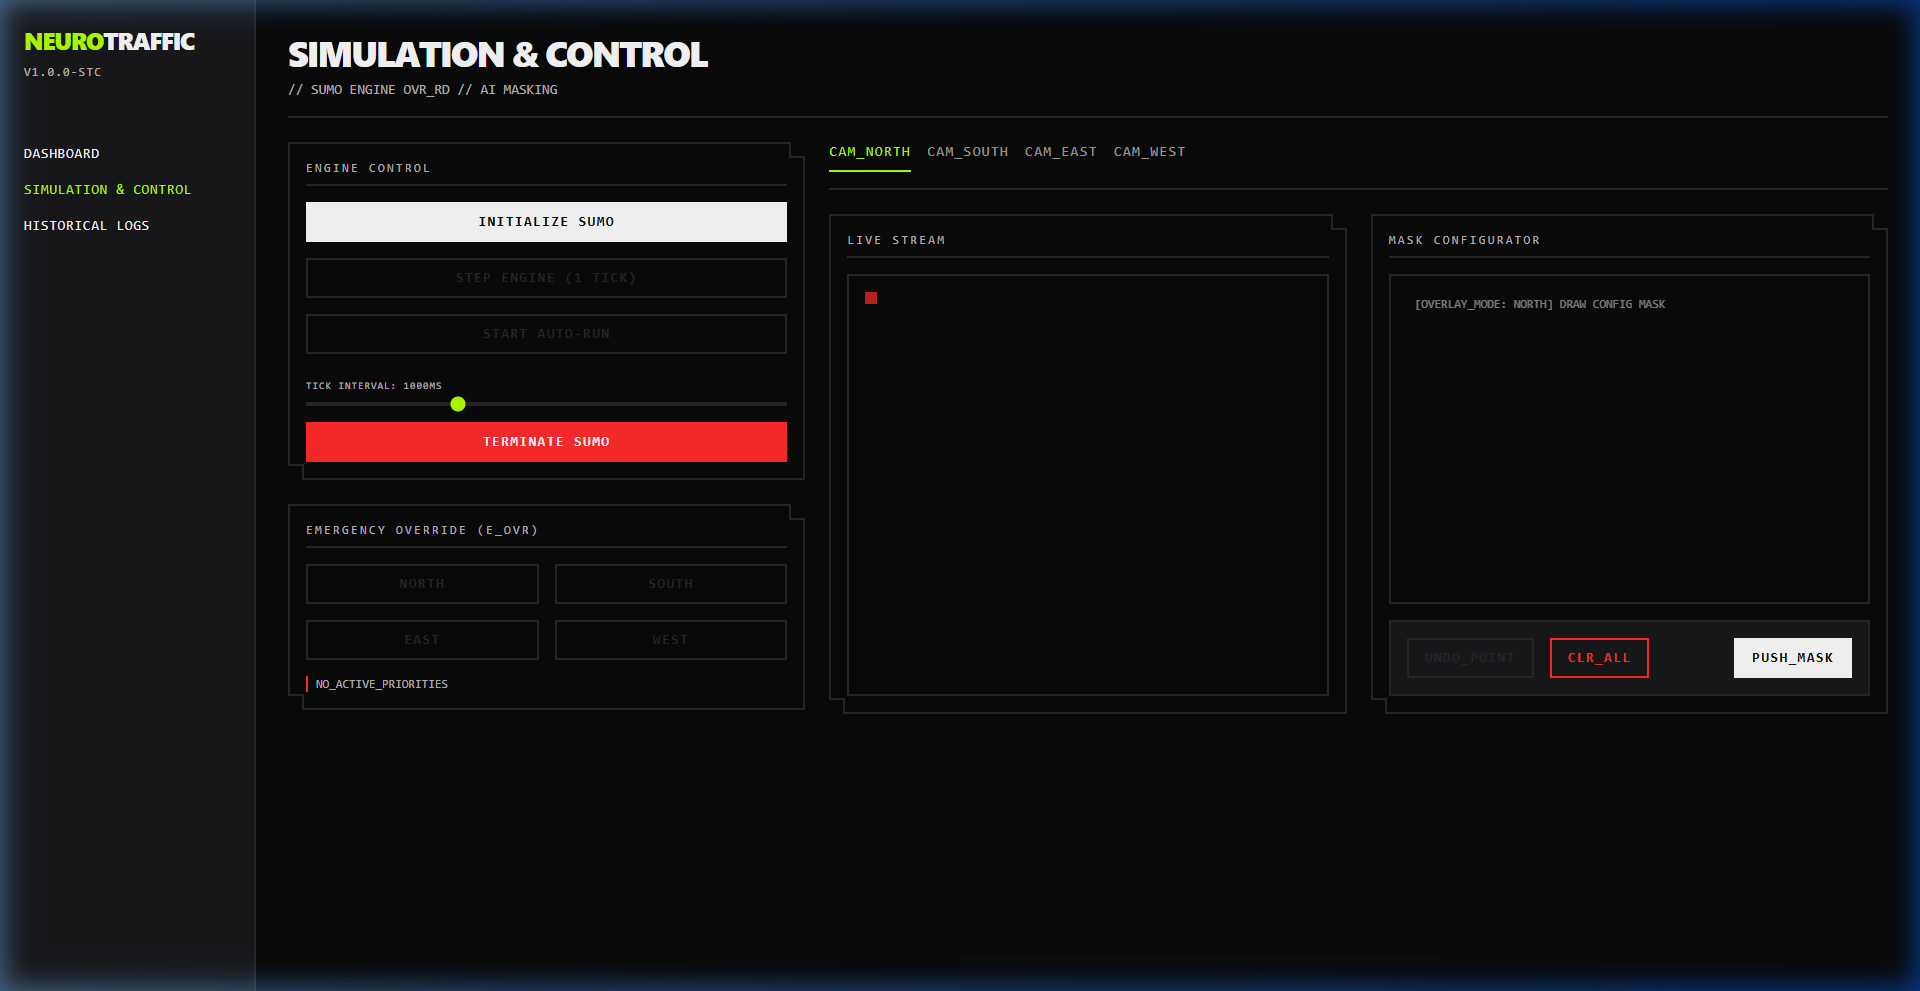
\includegraphics[width=0.9\textwidth]{screenshots/simulation_control.png}
    \caption{Simulation and Control Panel}
    \label{fig:sim_ctrl}
\end{figure}

\begin{figure}[H]
    \centering
    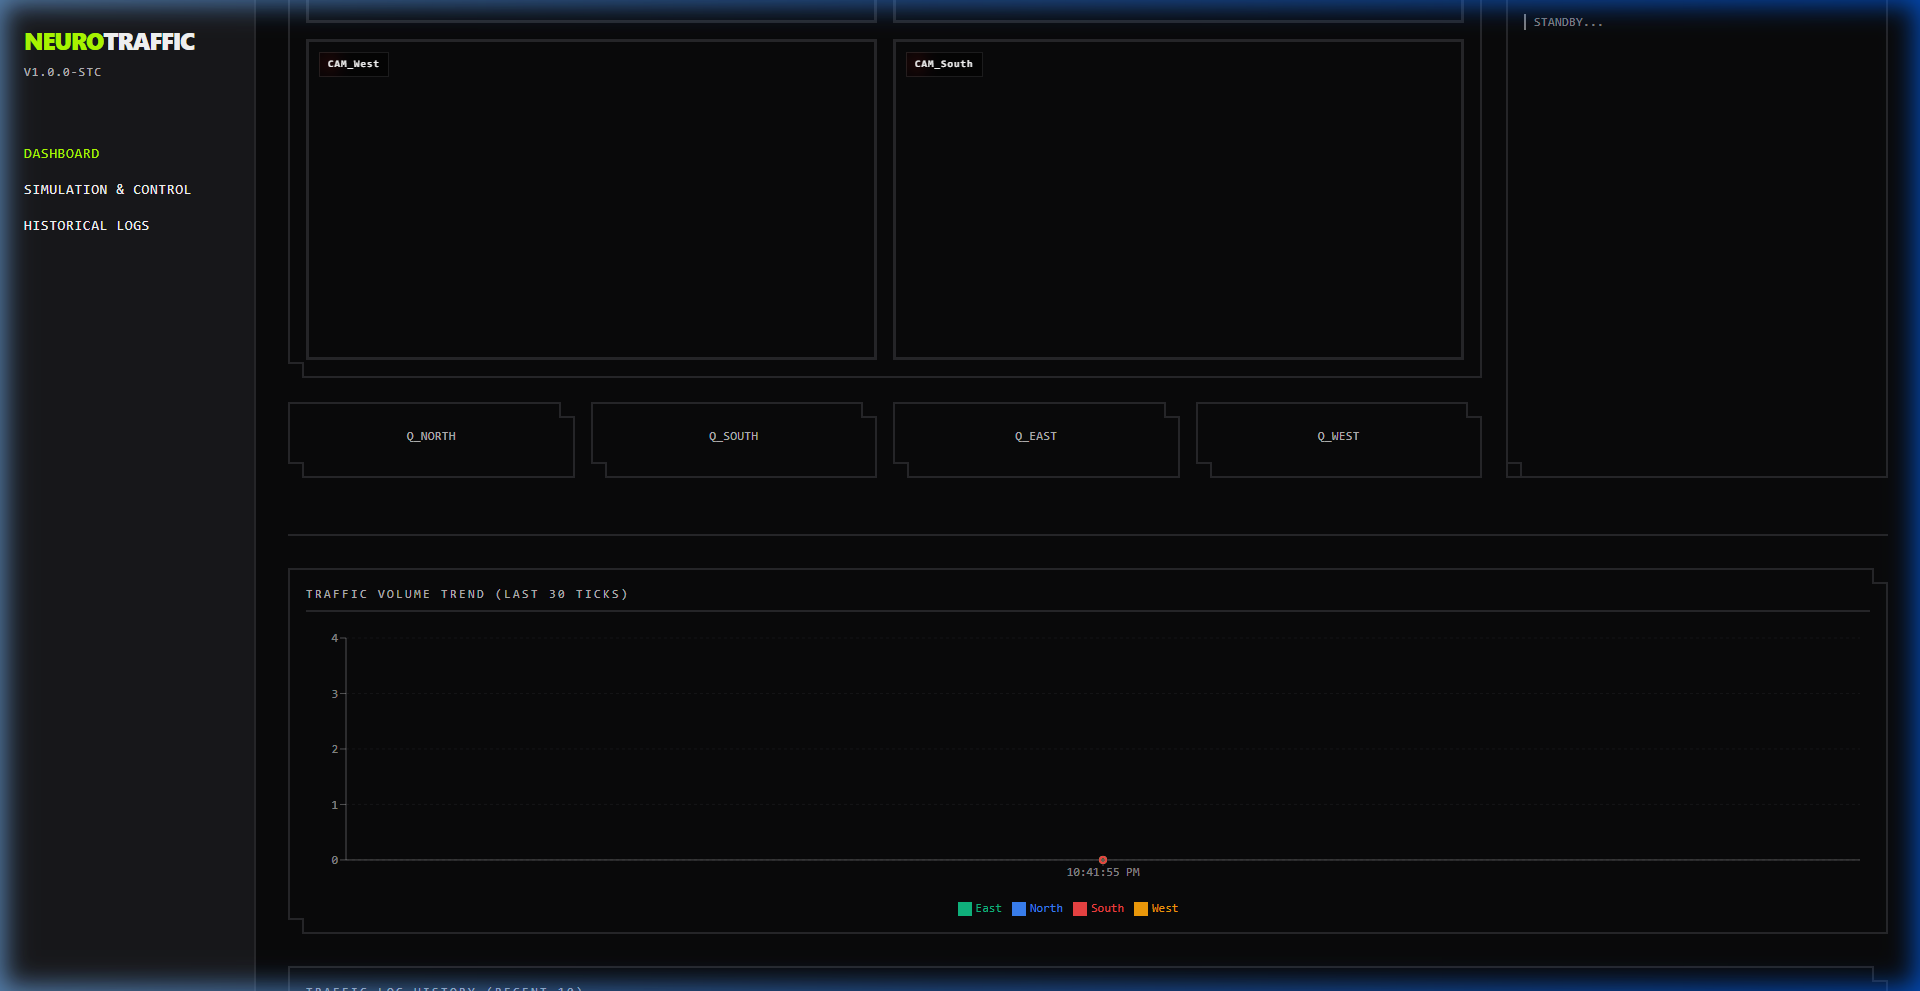
\includegraphics[width=0.9\textwidth]{screenshots/dashboard_charts.png}
    \caption{Real-time Traffic Volume Trends}
    \label{fig:charts}
\end{figure}

% --- Chapter 6: Conclusion ---
\chapter{Conclusion}
\section{Summary}
NeuroTraffic represents a significant step towards intelligent urban infrastructure. By leveraging modern AI techniques like YOLO26 and Reinforcement Learning, the system demonstrates that intersections can adapt dynamically to real-time demands. The integration with SUMO confirms the theoretical benefits in a controlled simulation, showing substantial improvements in traffic flow efficiency.

\section{Limitations}
\begin{itemize}
    \item \textbf{Hardware Dependency:} High-performance GPUs are required for real-time multi-camera processing, which might be a constraint for smaller municipalities.
    \item \textbf{Environmental Factors:} The current version of the YOLO model needs further validation under extreme weather conditions like heavy rain or fog.
\end{itemize}

\section{Future Work}
\begin{itemize}
    \item \textbf{Multi-Intersection Coordination:} Extending the RL agent to communicate with adjacent signals for city-wide synchronization.
    \item \textbf{V2X Integration:} Incorporating Vehicle-to-Infrastructure (V2I) communication for even more precise traffic data.
    \item \textbf{Edge Deployment:} Optimizing models for deployment on edge AI devices like NVIDIA Jetson.
\end{itemize}

% --- References ---
\begin{thebibliography}{99}
\bibitem{yolo} Ultralytics, "YOLO26: Real-time Object Detection," \url{https://github.com/ultralytics/ultralytics}.
\bibitem{fastapi} Tiangolo, "FastAPI framework, high performance, easy to learn, fast to code, ready for production," \url{https://fastapi.tiangolo.com/}.
\bibitem{sumo} P. A. Lopez et al., "Microscopic Traffic Simulation using SUMO," 2018 IEEE Intelligent Transportation Systems Conference (ITSC).
\bibitem{dqn} Mnih, V., et al., "Human-level control through deep reinforcement learning," Nature, 2015.
\bibitem{zang} Zheng, G., Zang, X., Xu, N., Wei, H., Yu, Z., et al., "Diagnosing Reinforcement Learning for Traffic Signal Control," arXiv preprint arXiv:1907.01948, 2019.
\bibitem{zhang_cityflow} Zhang, H., et al., "CityFlow: A Multi-Agent Reinforcement Learning Environment for Large Scale City-wide Traffic Signal Control," In \textit{Proceedings of the Web Conference (WWW)}, 2019.
\bibitem{react} Meta Open Source, "React -- A JavaScript library for building user interfaces," \url{https://react.dev/}.
\bibitem{pytorch} Meta AI, "PyTorch -- An open source machine learning framework," \url{https://pytorch.org/}.
\bibitem{tailwind} Tailwind Labs, "Tailwind CSS -- Rapidly build modern websites without ever leaving your HTML," \url{https://tailwindcss.com/}.
\bibitem{sqlite} SQLite Development Team, "SQLite -- Most used database engine in the world," \url{https://www.sqlite.org/index.html}.
\bibitem{aiortc} Jeremy Lainé, "aiortc -- WebRTC and ORTC implementation for Python using asyncio," \url{https://github.com/aiortc/aiortc}.
\bibitem{tanstack} TanStack, "TanStack Query -- Powerful asynchronous state management for TS/JS," \url{https://tanstack.com/query/latest}.
\end{thebibliography}

% --- Appendix ---
\appendix
\chapter{API Documentation}
NeuroTraffic exposes a wide range of endpoints for real-time data access, system configuration, and simulation control. The API is built using FastAPI and follows RESTful principles.

\section{Core Data Endpoints}
\begin{itemize}
    \item \textbf{GET /data} \\
    Returns the latest raw vehicle counts for each direction (North, East, West, South) as detected by the YOLO models.
    \item \textbf{GET /health} \\
    Checks the operational health of the backend, verifying that the RL models are loaded and the SUMO simulation is operational.
    \item \textbf{GET /summary} \\
    Generates a natural language summary of the current traffic state using a Large Language Model (LLM).
\end{itemize}

\section{Simulation \& Control Endpoints}
\begin{itemize}
    \item \textbf{GET /control/yolo} \\
    Retrieves the optimal traffic light action based on the live vehicle counts. Factors in emergency direction override if active.
    \item \textbf{GET /control/sumo/start | /step | /stop} \\
    Endpoints to manage the SUMO simulation lifecycle.
    \item \textbf{POST /control/emergency} \\
    Activates or deactivates emergency priority overrides. Requires a JSON payload with \texttt{direction} and \texttt{active} status.
\end{itemize}

\section{Historical Reporting Endpoints}
\begin{itemize}
    \item \textbf{GET /api/logs/traffic} \\
    Browse historical traffic volume logs stored in the SQLite database.
    \item \textbf{GET /api/logs/schedules} \\
    Browse historical traffic light signals and split schedules generated by the RL agent.
    \item \textbf{GET /api/logs/violations} \\
    Browse historical traffic violation logs (illegal parking, etc.).
\end{itemize}

\section{WebRTC Streaming}
\begin{itemize}
    \item \textbf{POST /offer} \\
    Accepts an SDP offer from a WebRTC client and returns an SDP answer to establish a peer-to-peer video stream of the annotated camera feed.
\end{itemize}

\end{document}